% no notes
%\documentclass{beamer}
% notes and slides
\documentclass[notes]{beamer}
% notes only
% \documentclass[notes=only]{beamer}
\usepackage{graphicx} % Allows including images
\usepackage{booktabs} % Allows the use of \toprule, \midrule and \bottomrule in tables
\usepackage{multirow}
\usepackage{multimedia}
\usepackage{url}
\usepackage{standalone}
\usepackage{adjustbox}
\usepackage{lmodern}
\usepackage{pgfplots}
\usepackage{amsmath}
\usepackage{amsthm}
\usepackage{multimedia}
\usepackage{media9}

% plotting.
\usepackage{standalone}
\usepackage{tikz}
\usepackage{pgfplots}
\usepgfplotslibrary{groupplots,dateplot}
\usetikzlibrary{patterns,shapes.arrows}
\pgfplotsset{compat=newest}

\usepackage{csquotes}


\PassOptionsToPackage{american}{babel} % change this to your language(s), main language last
% Spanish languages need extra options in order to work with this template
% \PassOptionsToPackage{spanish,es-lcroman}{babel}
\usepackage{babel}

\PassOptionsToPackage{%
  backend=biber,bibencoding=utf8, %instead of bibtex
  %backend=bibtex8,bibencoding=ascii,%
  language=auto,%
  style=numeric-comp,%
  %style=authoryear-comp, % Author 1999, 2010
  %bibstyle=authoryear,dashed=false, % dashed: substitute rep. author with ---
  style=alphabetic,
  sorting=nyt, % name, year, title
  maxbibnames=10, % default: 3, et al.
  %backref=true,%
  %natbib=true % natbib compatibility mode (\citep and \citet still work)
}{biblatex}
\usepackage{biblatex}

\addbibresource{bib.bib}

\usetheme{metropolis}           % Use metropolis theme
\setbeamertemplate{caption}[default]
\title{Optimization for Machine Learning in Python}
\institute{High-Performance Computing and Analytics Lab, Uni Bonn}
\author{Dr. Moritz Wolter}
\date{\today}

\titlegraphic{
\includegraphics[width=2.00cm]{UNI_Bonn_Logo_Standard_RZ.pdf}}
\begin{document}
    \maketitle

    \begin{frame}
    \frametitle{Overview} 
    \tableofcontents
    \end{frame}

    \section{Introduction}
    \begin{frame}{Optimization}
      Traditionally, optimization means minimizing using a cost function $f(x)$.
      Given the cost, we must find the cheapest point $x^*$ on the function,
      or in other words,
      \begin{align}
       x^* = \min_{x \in \mathbb{R}} f(x)        
      \end{align}
    \end{frame}

    \begin{frame}{Functions}
      Functions are mathematical mappings. Consider for example, the quadratic function,
      $f(x): \mathbb{R} \rightarrow \mathbb{R}$:
      \begin{align}
        f(x) = x^2
      \end{align}

    \begin{figure}
      \includestandalone[scale=.7]{./figures/parabola}
    \end{figure}
    \end{frame}

    \begin{frame}{Where is the minimum?}
      \begin{figure}
        \includestandalone[scale=.7]{./figures/parabola}
      \end{figure}
      In this case, we immediately see it's at zero. To find it via an iterative process, we require derivate information.
    \end{frame}

    \begin{frame}{Summary}
      \begin{itemize}
        \item Functions assign a value to each input.
        \item We seek an iterative way to find the smallest value.
        \item Doing so requires derivates.
      \end{itemize}
    \end{frame}

    \section{The derivative}
    \begin{frame}{The derivative}
      \begin{align}
        \dfrac{d f(x)}{dx} = \lim_{h \rightarrow 0} \dfrac{f(x + h) - f(x)}{h}
      \end{align}
      \begin{figure}
        \includestandalone[scale=.7]{./figures/parabola_derivative}
      \end{figure}
    \end{frame}

    
    \begin{frame}{Derivation of the parabola derivative}
      \begin{align}
          \lim_{h \rightarrow 0} \dfrac{(x + h)^2 - x^2}{h} 
          & = \lim_{h \rightarrow 0} \dfrac{x^2 + 2xh + h^2 - x^2}{h}   \\
          & = \lim_{h \rightarrow 0} \dfrac{2xh + h^2}{h}  \\
          & = \lim_{h \rightarrow 0} \dfrac{h (2x + h)}{h}  \\
          & = \lim_{h \rightarrow 0} 2x + h \\
          & = 2x
      \end{align}
      \note{Derive on the board:
          \begin{align}
            \lim_{h \rightarrow 0} \dfrac{(x + h)^2 - x^2}{h} 
            & = \lim_{h \rightarrow 0} \dfrac{x^2 + 2xh + h^2 - x^2}{h}   \\
            & = \lim_{h \rightarrow 0} \dfrac{2xh + h^2}{h}  \\
            & = \lim_{h \rightarrow 0} \dfrac{h (2x + h)}{h}  \\
            & = \lim_{h \rightarrow 0} 2x + h \\
            & = 2x
        \end{align}
      }
    \end{frame}

    \begin{frame}{Summary}
      \begin{itemize}
        \item A function is differentiable if the limit of the difference quotient exists.
        \item For any point on a differentiable function, the derivative provides a tangent slope.
        \item We will exclusively work with differentiable functions in this course.
      \end{itemize}
    \end{frame}

    \section{Optimization in a single dimension}
    \begin{frame}{Steepest descent}
      To find a minimum, we descent along the gradient, with $n$ denoting the step number,
      $\epsilon \in \mathbb{R}$ the step size and $\dfrac{d f}{dx}$ the derivate of $f$ along 
      $x \in \mathbb{R}$:
      \begin{align}
        x_n = x_{n-1} - \epsilon \cdot \dfrac{d f}{dx}.
      \end{align}
    \end{frame}


    \begin{frame}{Steepest descent on the parabola}
      Working with the initial position $x_0 = 5$ and a step size of $\epsilon = 0.1$ for $25$ steps leads to: 
      \begin{figure}
        \includestandalone[width=0.475\linewidth]{./figures/parabola_opt}
        \includestandalone[width=0.49\linewidth]{./figures/f_prime_1d}
      \end{figure}
    \end{frame}

    \begin{frame}{Summary}
      \begin{itemize}
        \item Following the negative derivative iteratively got us to the minimum.
        \item At points of interest, the first derivate is zero. 
      \end{itemize}
    \end{frame}

    \section{Optimization in many dimensions}

    \begin{frame}{The two-dimensional paraboloid}
      \begin{align}
        f(x_1, x_2) = x_1^2 + x_2^2
      \end{align}
      \begin{figure}
        \centering
        \includestandalone[scale=.8]{./figures/paraboloid}
      \end{figure}
    \end{frame}

    \begin{frame}{The gradient}
      The gradient lists partial derivatives with respect to all inputs in a vector.
      For a function $f : \mathbb{R}^n \rightarrow \mathbb{R}$ of $n$ variables the gradient
      $\nabla f: \mathbb{R}^n \rightarrow \mathbb{R}^n$ is defined as
      \begin{align}
        \nabla f = \begin{pmatrix}
          \frac{\partial f}{\partial x_1} \\
          \frac{\partial f}{\partial x_2} \\
          \vdots \\
          \frac{\partial f}{\partial x_n} 
        \end{pmatrix}.
      \end{align}
      \note{
        \begin{itemize}
          \item Gradients point in the steepest ascent direction.
          \item To find the gradient, we must compute the partial derivate with respect to every input.
          \item A vector collects all derivates.
        \end{itemize}
      }
    \end{frame}

    \begin{frame}{Computing the gradient of the paraboloid}
      \begin{align}
        \nabla f(x_1, x_2) &= \nabla (x_1^2 + x_2^2) \\
                           &= \begin{pmatrix}
                              2x_1 \\
                              2x_2
                              \end{pmatrix}
      \end{align}
    \end{frame}

    \begin{frame}{Gradients at points}
      For every point $\mathbf{p} = (x_1, x_2, \dots , x_n)$ we can write
      \begin{align}
        \nabla f (\mathbf{p}) = \begin{pmatrix}
          \frac{\partial f}{\partial x_1} (\mathbf{p}) \\
          \frac{\partial f}{\partial x_2} (\mathbf{p}) \\
          \vdots \\
          \frac{\partial f}{\partial x_n} (\mathbf{p}) 
        \end{pmatrix}.
      \end{align}
    \end{frame}


    \begin{frame}{Gradients on the Paraboloid}
      \begin{figure}
        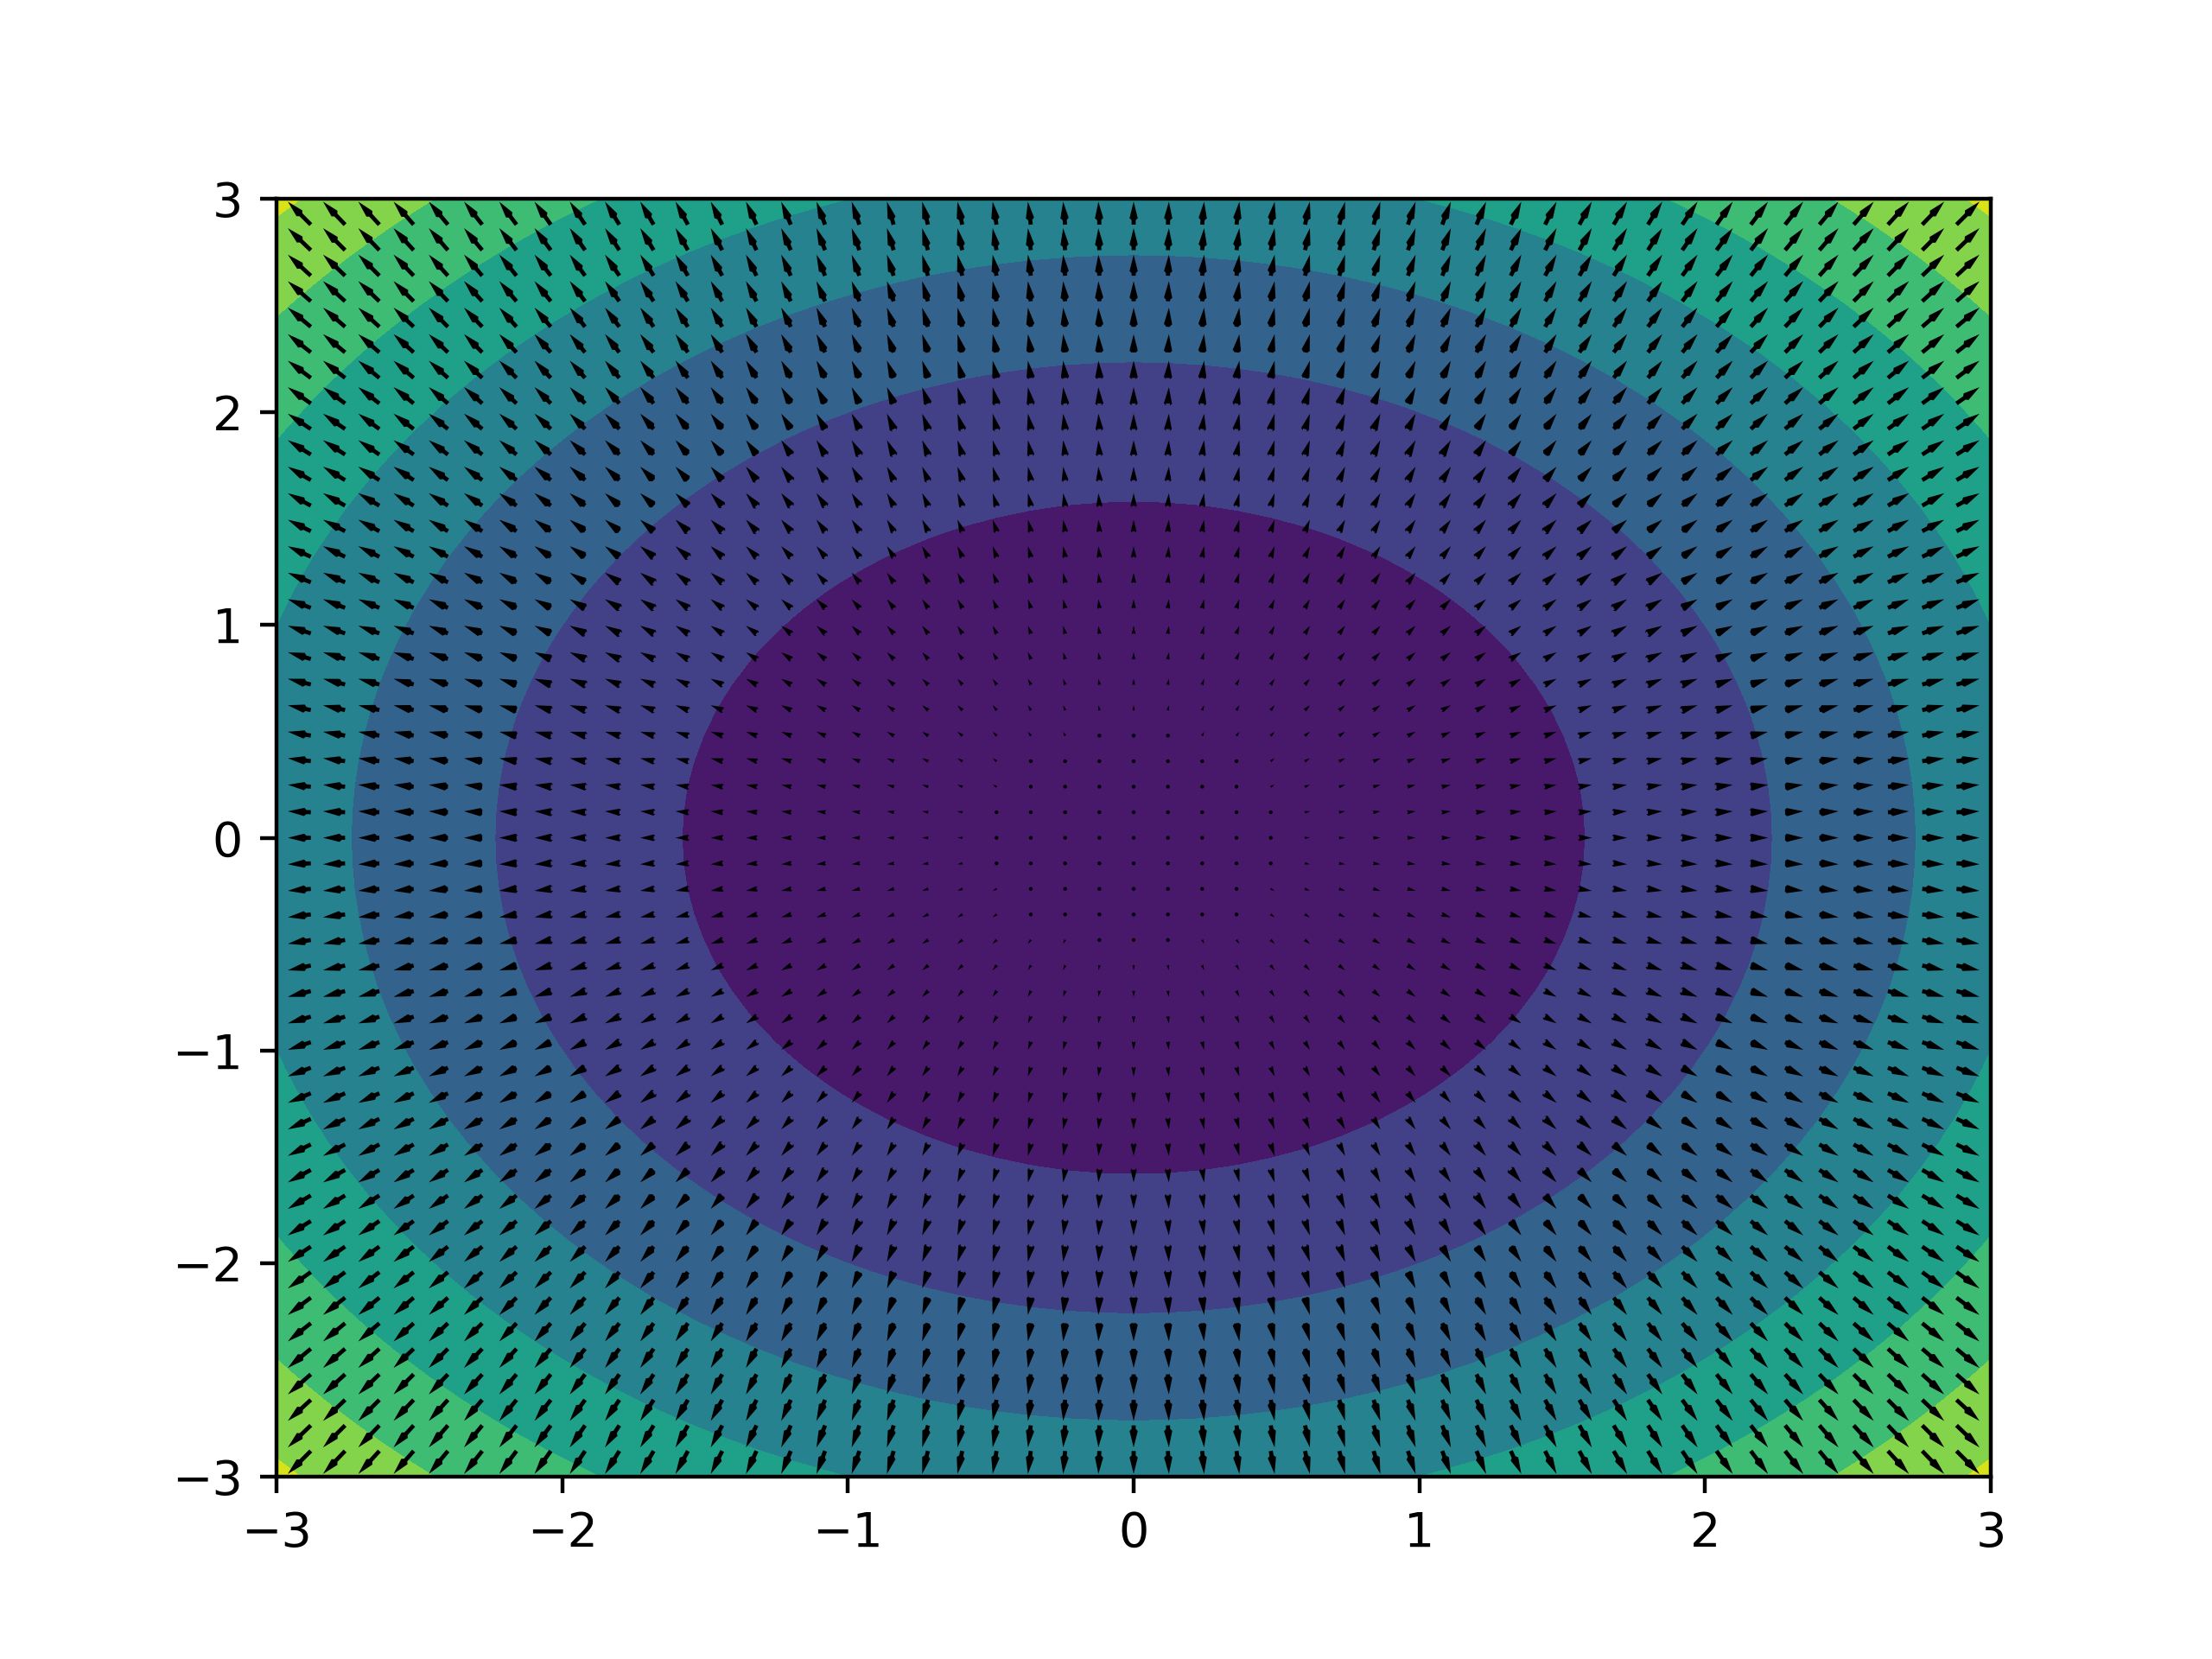
\includegraphics[width=.9\linewidth]{./figures/quiver_paraboloid.png}
      \end{figure}
    \end{frame}

    \begin{frame}{Gradient descent}
      Initial position: $x_0 = [2.9, -2.9]$, \\
      Gradient step size: $\epsilon = 0.025 $
      \begin{align}
        x_n = x_{n-1} - \epsilon \cdot \nabla f(\mathbf{x})
      \end{align}
      $n$ denotes the step number, $\nabla$ the gradient operator, and $f(\mathbf{x})$ a vector valued function.
    \end{frame}

    \begin{frame}{Gradient descent on the Paraboloid}
      \centering
      \movie[width=6.4cm,height=4.8cm,poster]{Paraboloid Optimization}{paraboloid_descent.mp4}
    \end{frame}

    \begin{frame}{The Rosenbrock test function}
      \begin{align}
        f(x_1, x_2) = (a - x_1)^2 + b(x_2 - x_1^2)^2
      \end{align}
      \begin{figure}
        \includestandalone[scale=0.7]{./figures/rosenbrock}
        \caption{Rosenbrock function with a=1 and b=100 .}
      \end{figure}
    \end{frame}

    \begin{frame}{The gradient of the Rosenbrock function}
      Recall the Rosenbrock function:
      \begin{align}
        f(x, y) = (a - x)^2 + b(y - x^2)^2 \\
        \nabla f(x, y) = \begin{pmatrix}
          -2a + 2x - 4byx + 4bx^3 \\
          2by - 2bx^2 \\
        \end{pmatrix}
      \end{align}
      \note{
      On the board, derive:
      \begin{align}
        f(x,y) &= (a - x)^2 + b(y-x^2)^2 \\
               &= a^2 - 2ax + x^2 + b(y^2 - 2yx^2 + x^4) \\
               &= a^2 - 2ax + x^2 + by^2 - 2byx^2 + bx^4 \\
        \Rightarrow \dfrac{\partial f(x,y)}{\partial x} &= -2a + 2x - 4byx + 4bx^3 \\
        \Rightarrow \dfrac{\partial f(x,y)}{\partial y} &= 2by - 2bx^2
      \end{align}
      }
    \end{frame}

    \begin{frame}{Gradients on the Rosenbrock function}
      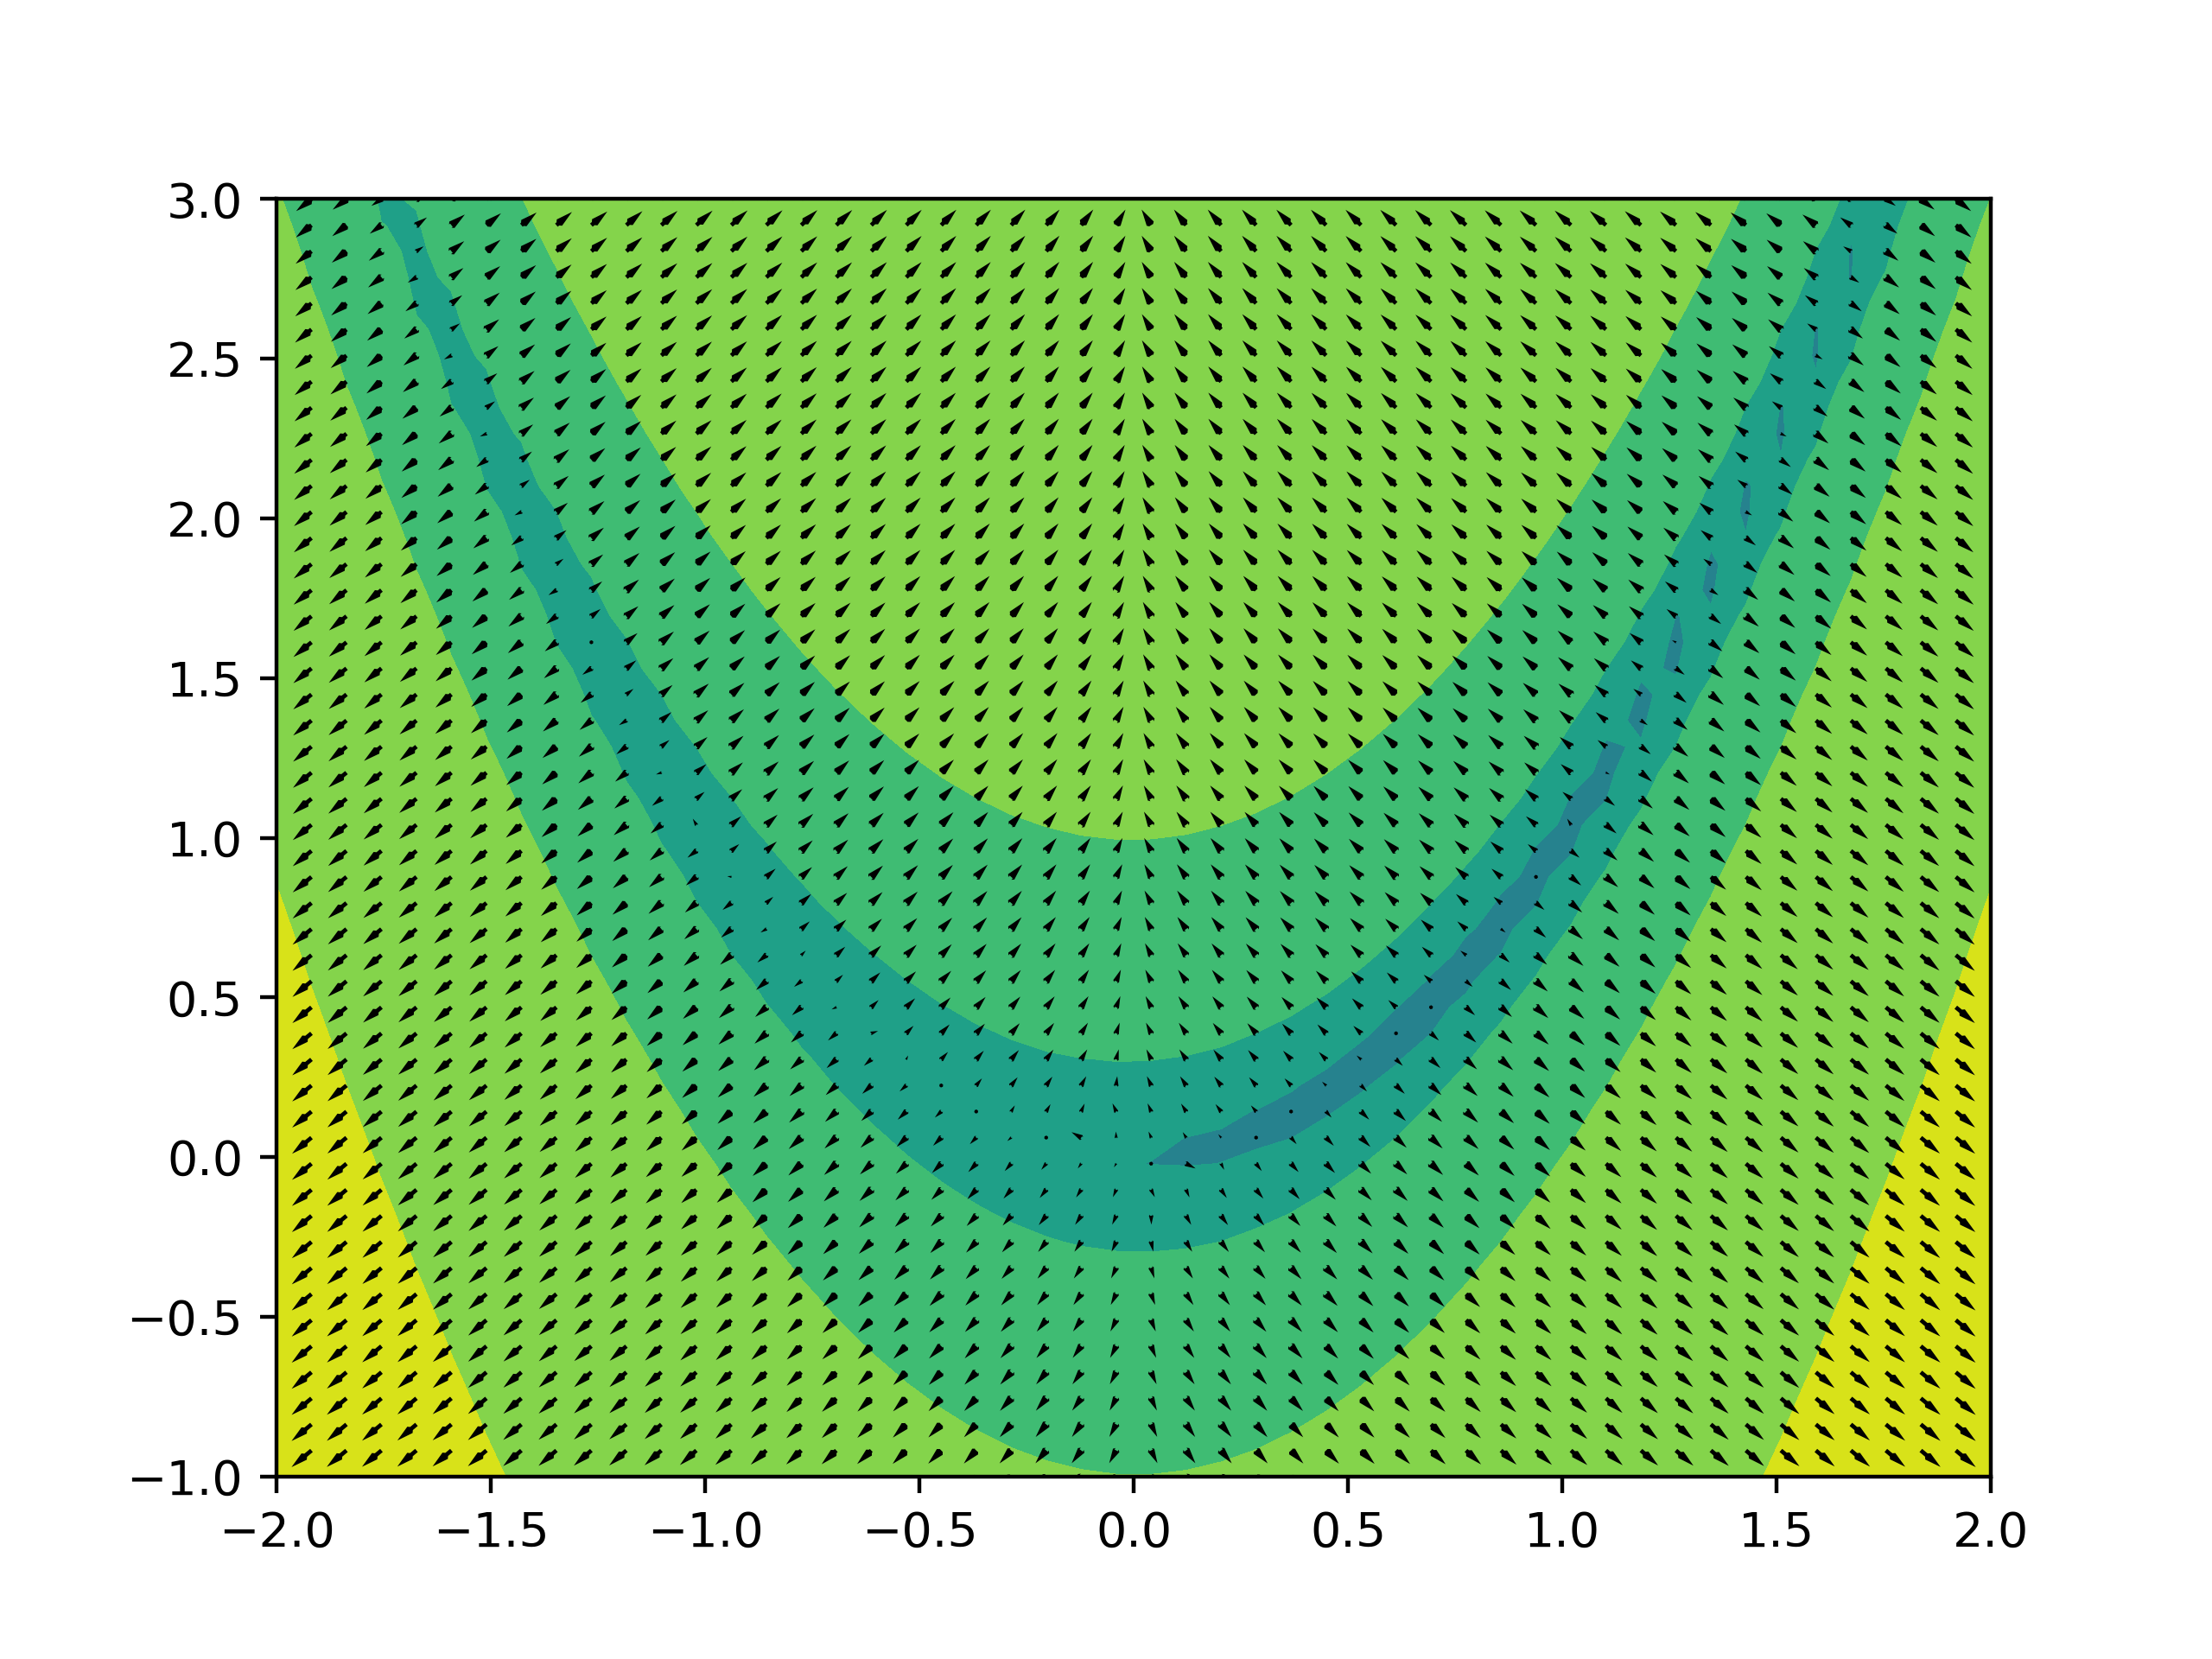
\includegraphics[width=.9\linewidth]{./figures/quiver.png}
    \end{frame}

    \begin{frame}{Gradient descent}
      Initial position: $x_0 = [0.1, 3.]$, \\
      Gradient step size: $\epsilon = 0.01 $
      \begin{align}
        \mathbf{x}_n = \mathbf{x}_{n-1} - \epsilon \cdot \nabla f(\mathbf{x})
      \end{align}
      $n$ denotes the step number, $\nabla$ the gradient operator, and $f(\mathbf{x})$ a vector valued function.
    \end{frame}

    \begin{frame}{Gradient descent on the Rosenbrock function}
      \centering
      \movie[width=6.4cm,height=4.8cm,poster]{Rosenbrock Optimization}{rosenbrock_momentum_0.0.mp4}
    \end{frame}

    \begin{frame}{Motivating Momentum}
      \begin{itemize}
        \item The standard gradient descent approach gets stuck.
        \item What if we could somehow use a history of recent gradient information?
      \end{itemize}
    \end{frame}

    \begin{frame}{Gradient descent with momentum}
      Initial position: $x_0 = [0.1, 3.]$, \\
      Gradient step size: $\epsilon = 0.01 $, \\
      Momentum parameter: $\alpha = 0.8$
      \begin{align}
        \mathbf{v} &= \alpha \mathbf{v}_{n-1} - \epsilon \cdot \nabla f(\mathbf{x}) \\
        \mathbf{x}_n &= \mathbf{x}_{n-1} + \mathbf{v}
      \end{align}
      $\mathbf{v}$ denotes the velocity vector, 
      $n$ the step number, $\nabla$ the gradient operator, and $f(\mathbf{x})$ a vector-valued function.
    \end{frame}


    \begin{frame}{Gradient descent with momentum}
      \centering
      \movie[width=6.4cm,height=4.8cm,poster]{Rosenbrock Optimization}{rosenbrock_momentum_0.8.mp4}
    \end{frame}

    %\begin{frame}{Automatic gradients}
    % TODO 
    %\end{frame}

    \begin{frame}{Summary}
      \begin{itemize}
        \item Gradient descent works in high-dimensional spaces!
        \item On the Rosenbrock function, we required momentum to find the minimum.
        \item Momentum adds the notion of inertia, which can help overcome local minima in some cases.
        \item Just like in the 1d case, the gradient equals zero at local minima and saddle points.
      \end{itemize}
    \end{frame}

    \section{Optimization for deep learning}
    \begin{frame}{The chain rule}
    %    TODO
    \end{frame}


    \begin{frame}[allowframebreaks]{Optional reading}
      \begin{itemize}
        \item Mathematics for machine learning, \cite[Chapter 5, Vector Calculus]{deisenroth2020mathematics}
        \item Deep learning, \cite[Chapter 8.2, Automatic Differentiation]{wright1999numerical}
        \item Numerical optimization, \cite[Chapter 8, Optimization for Training Deep Models]{goodfellow2016deep}
      \end{itemize}
    \end{frame}

    \begin{frame}
      \frametitle{References}
      \renewcommand*{\bibfont}{\scriptsize}
      \setbeamertemplate{bibliography item}{\insertbiblabel}
      \printbibliography
  \end{frame}

\end{document}
